\documentclass[12pt]{article}
\usepackage[utf8]{inputenc}
\usepackage[dutch]{babel}
\usepackage{algorithm}
\usepackage{algorithmic}
\usepackage{amssymb}
\usepackage{amsmath}
\usepackage{graphicx}

\author{Wolfgang M\"ollmann \& Robbe Degr\`eve}
\title{Toepassingen van meetkunde in de informatica \\ Project: Bepaling van het Dichtste Puntenpaar}

\begin{document}

\maketitle

\newpage

\section{Beschrijving van opstelling van puntenverzameling}
Voor het opstellen van een input-file met een aantal gegeven parameters om willekeurge punten te creëren gebruiken we de functie "makeRandom".
Deze functiezal de volgende parameters als input vragen:
\begin{enumerate}
    \item inFile: De puntenverzameling zal in dit bestand weggeschreven worden, indien het bestand niet bestaat zal het aangemaakt worden.
    \item alg: het nummer van het algoritme dat gebruikt moet worden: 1 (eenvoudige algoritme), 2 (eerste variante van het doorlooplijnalgoritme) of 3 (tweede variante van het doorlooplijnalgoritme)
    \item dim: de dimensie van de punten $M \geq 2$
		\item size: het aantal punten N
\end{enumerate}

Deze functie heeft als taak om een inputbestand op te stellen met willekeurge co\"ordinaten.
De functie zal de gegeven parameters eerst neerschrijven in de inFile.
Daarna gebeurd een initialisatie van \texttt{Random r}.
Daarna zullen we per regel van het bestand itereren van 0 tot en met de dimensie en voor iedere dimensie een willekeurige waarde neerschrijven in het bestand.
De willeukeurige co\"ordinaten kunnen waardes aannemen tussen $[0, 5[$.

Voor de \textit{worst-case} puntenverzameling voor de eerste variant van het doorlooplijnalgoritme voor M = 2 hebben we een javafunctie \texttt{makeWorstCase}.
In deze functie maken een puntenverzameling aan van één kolom, waarbij alle punten dezelfde x-waarde hebben.
De y-waarde speelt hierbij geen rol.
In onze rij-implementatie sorteren we de punten met dezelfde x-waarden volgens de y-waarde.
Het tweede punt zal dus enkel vergelijken met het punt boven hem.
Het derde punt zal nadien vergelijken met het eerste en het tweede punt.
Uiteindelijk zal het laatste (onderste) punt zal dus met alle punten vergelijken.
Dit zal ons uiteindelijk $\frac{(n+1)}{2}$ vergelijkingen geven. De complexiteit zal dus $O(n^2/2)$ zijn.


\begin{algorithm}
\caption{De javafunctie \texttt{makeRandom}}
\begin{algorithmic}
\STATE \textbf{Input:} $inFile$, $alg$, $dim$, $size$
\STATE infile.println(alg)
\IF {$dim < 2$}
	\PRINT Dimension needs to be greater or equal to 2.
	\STATE \texttt{Exit}
\ENDIF
\STATE Random r = new Random()
\STATE $Iterator<Double> i$ = r.doubles(size * dim, 0.0, 5.0).iterator()
\STATE $String outString = ""$
\WHILE {$i.hasNext()$}
	\STATE $outString = ""$
	\FOR {$j = 0$; $j < dim$; j++}
		\STATE outString += String.format(Locale.US, "\%17.16f ", i.next())
	\ENDFOR
	\STATE inFile.println($outString$)
\ENDWHILE
\STATE inFile.flush()
\STATE inFile.close()
\end{algorithmic}
\end{algorithm}

\section{Opdracht 1: Hoog-niveau beschrijving van verscheidene algoritmes}

\subsection{Brute-force algorithm}

\subsubsection{hoogniveau beschrijving}

\begin{algorithm}
\caption{Bereken het dichtste puntenpaar met brute-force}
\begin{algorithmic}
	\STATE \textbf{Input:}  $rij$: Array met $N$ punten (gesorteerd naar stijgende x-co\"ordinaat)
  \STATE $d$ = $+\infty$
	\STATE $dpp1$ = 0, $dpp2$ = 0
  \STATE $currentDist$ = 0
  \FOR {$i$ to $length(rij)-1$}
    \FOR {$j = i + 1$ to $length(rij)$}
      \STATE $currentDist$ = calculate\_dist($rij[i]$, $rij[j]$)
      \IF {$currentDist < d$}
				\STATE $dpp1$ = $rij[i]$
				\STATE $dpp2$ = $rij[j]$
        \STATE $d$ = $currentDist$
  		\ENDIF
    \ENDFOR
  \ENDFOR
  \RETURN $dpp1$, $dpp2$, $d$
\end{algorithmic}
\end{algorithm}

\newpage
\subsection{Variant 1 algorithm}
\subsubsection{hoogniveau beschrijving}


\begin{algorithm}
\caption{Bereken het dichtste Puntenpaar volgens variant 1}
\begin{algorithmic}
	\STATE \textbf{Input:}  $rij$: Array met $N$ punten (gesorteerd naar stijgende x-co\"ordinaat)
	\STATE $d$ = $+\infty$
	\STATE $dpp1$ = 0, $dpp2$ = 0
	\STATE $currentDist$ = 0
	\FOR {$i = 1$ to $length(rij)$}
		\FOR {$j = i - 1$ to $0$}
		\IF {$rij[i].x - rij[j].x > d$}
			\STATE $break$
		\ENDIF
		\STATE $currentDist$ = calculate\_dist($rij[i]$, $rij[j]$)
			\IF {$currentDist < d$}
				\STATE $dpp1$ = $rij[i]$
				\STATE $dpp2$ = $rij[j]$
				\STATE $d$ = $currentDist$
			\ENDIF
		\ENDFOR
	\ENDFOR
	\RETURN $dpp1$, $dpp2$, $d$
\end{algorithmic}
\end{algorithm}

\subsection{Variant 2 algorithm}
\subsubsection{hoogniveau beschrijving}

\begin{algorithm}
\caption{Bereken het dichtste Puntenpaar volgens variant 2}
\begin{algorithmic}
	\STATE \textbf{Input:}  $rij$: Array met $N$ punten (gesorteerd naar stijgende x-co\"ordinaat)
	\STATE $d$ = $+\infty$
	\STATE $dpp1$ = 0, $dpp2$ = 0
	\STATE $currentDist$ = 0
	\STATE $t$: gegevensstructuur waarin punten links van de doorlooplijn opgeslagen zijn, gesorteerd naar stijgende y-coordinaat


\end{algorithmic}
\end{algorithm}

\section{Grafieken}

In Figuur 1 zullen we de rekentijden tussen het brute-force algoritme en variant1 vergelijken.
We zullen op de x-as het aantal punten uitzetten.
% Deze 302 komt eigenlijk omdat ik van 250 ben begonnen -> 275 -> 302, maar onder 300 gaf was omdat
% wel een beetje afwijkend van de verwachte rechte
De gekozen aantal punten zijn logaritmisch bepaald met als basis 1.1 beginnend vanaf 302 tot en met 12279.
% TODO Waarom gekozen voor log met b=1.1 => Echt puur voor meer datapunten te hebben zonder dat ik uren moet wachten
Op de y-as zetten we de rekentijd uit in milliseconden. Hiervoor gebruiken we een logaritmische functie met basis 2.
% TODO wel verband precies kunnen we concluderen (lineair, expo, ...)
% Goeie vraag, ze lijken allebei FACTOR * N^2 te zijn niet? met die base 2 voor het logaritme?
We kunnen concluderen uit deze plot dat variant 1 voor alle onze gekozen punten een effeciënter algoritme is.
We kunnen ook zien dat de het brute-force algoritme een steiler verloop heeft, hieruit kunnen we afleiden dat voor zeer grote aantallen punten het verschil tussen de twee algoritmes steeds groter worden.

\begin{figure}
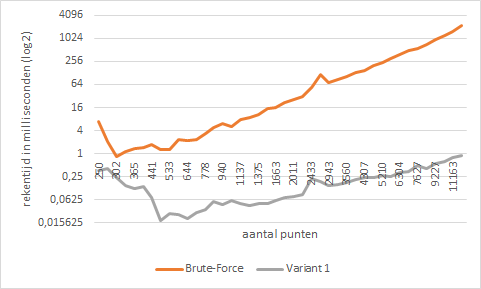
\includegraphics[width=\textwidth]{Simpel-var1-rekentijd.png}
\caption{De plot van de rekentijden tussen het brute-force algoritme en variant 1}
\end{figure}

In figuur 2 zullen we het verband tussen de Kmax en het aantal punten plotten.
Op de x-as zetten we het aantal punten uit van 250 tot 12279 met een logaritmische functie met basis 1,1.
Op de y-as zetten we de Kmax uit die in dit geval zal gaan van een minimum van 2 tot en met een maximum van 25.
We kunnen op de plot zien dat de grafiek Kmax een licht stijgend karakter heeft.

\begin{figure}
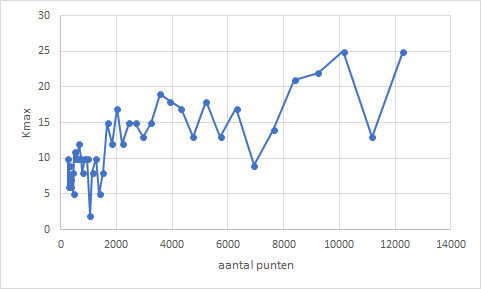
\includegraphics[width=\textwidth]{punten-Kmax.png}
\caption{De plot tussen het aantal punten en Kmax}
\end{figure}

In figuur 3 zullen we het verband tussen de Kavg en het aantal punten plotten.
Op de x-as zetten we het aantal punten uit van 250 tot 12279 met een logaritmische functie met basis 1.1.
Op de y-as zetten we de Kmax uit die in dit geval zal gaan van een minimum van 0,1480 tot en met een maximum van 2,14186.
Op deze plot is duidelijk te herkennen dat Kavg ongeveer constant zal blijven ongeacht het aantal punten.
In ons experiment was deze constante rond 1,35.

\begin{figure}
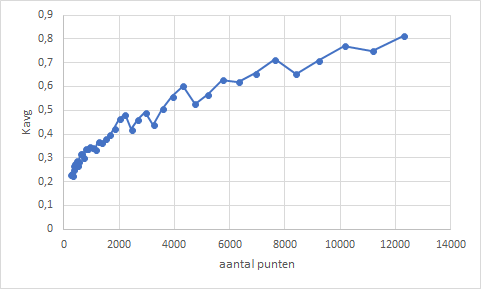
\includegraphics[width=\textwidth]{punten-Kavg}
\caption{De plot tussen het aantal punten en Kavg}
\end{figure}

In Figuur 4 zullen we de het aantal dimensies plotten in functie van de rekentijd voor variant 1.
We zullen op de x-as het aantal dimensies uitzetten van 2 tot en met 19.
Op de y-as zetten we de rekentijd uit in milliseconden.


\begin{figure}
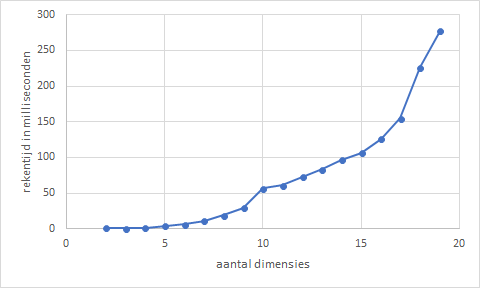
\includegraphics[width=\textwidth]{dim-var1-rekentijd.png}
\caption{De plot tussen het aantal dimensies en de rekentijd van variant 1 (voor 2500 punten)}
\end{figure}

\begin{figure}
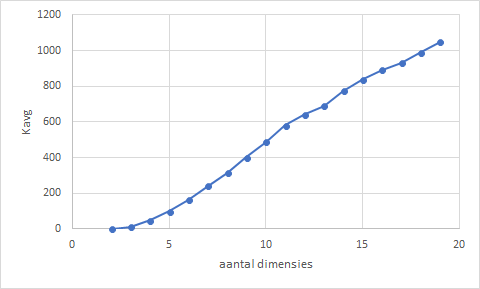
\includegraphics[width=\textwidth]{dim-Kavg.png}
\caption{De plot tussen het aantal dimensies en Kavg (voor 2500 punten)}
\end{figure}







\end{document}
